\chapter{Editing Metamaterial Devices}
\label{chapter:software}

\todo{write short intro: editors give lots of freedom... for exploring because they're new...}

To allow users to design, fabricate, and test metamaterials containing mechanisms we implemented the specialized editor shown in Figure \ref{fig:20-editor-ui}. 

\begin{figure} [h]
    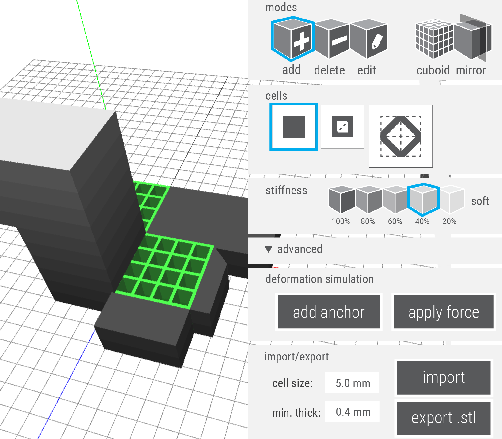
\includegraphics[width=\textwidth]{chapters/metamaterial-mechanisms-FIG/20-editor-ui.pdf}
    \caption[Short figure name.]{Our editor allows users to edit and simulate the deformation of metamaterial mechanisms interactively. 
    \label{fig:20-editor-ui}}
\end{figure}

The main intent behind it is not only to make the editing process more efficient than the more traditional script-based editing, but also to provide users with an overview of their design, encouraging design by trial-and-error. 

Our editor is based on interaction techniques known from voxel editors (such  as \cite{VoxCAD2018}). However, in addition our software also offers specific supports for creating mechanisms, such as tools for drawing hinge arrays, etc. In order to allow users to validate their designs, the editor also allows them to apply forces and see how the object deforms in order to then refine their design directly inside the editor, before exporting to the 3D printer.

%\section{Encapsulating domain knowledge into the editor}


%-----------------MECHANISMS-----------------

\section{Editing metamaterial mechanisms}

\subsection{User interaction}

Figure \ref{fig:21-editor-walkthrough} illustrates how users create the door handle example.

(a) Users start by creating a block of rigid cells using the \textit{add brush}. They can remove cells using the \textit{delete brush}. Here, users utilize the tool in \textit{cuboid mode}, which allows them to draw a filled rectangular region at once by just drawing the diagonal. (b) By adding another two cuboids on top, users create the handle.

(c) Next, Users select the \textit{shear brush}. Still in cuboid mode, they paint the central hinge array using a single drag interaction, which causes rigid cells to turn into shear cells. Even though the block of material that users painted on is two cells high, the shear brush paints cells all the way through---as they can tell from the sidewall now being all green. This is one of the features of this brush: since shear cells backed by rigid cells would still be rigid, thus have no effect, the shear brush always cuts shear cells through the entire object. 

\begin{figure} [h]
    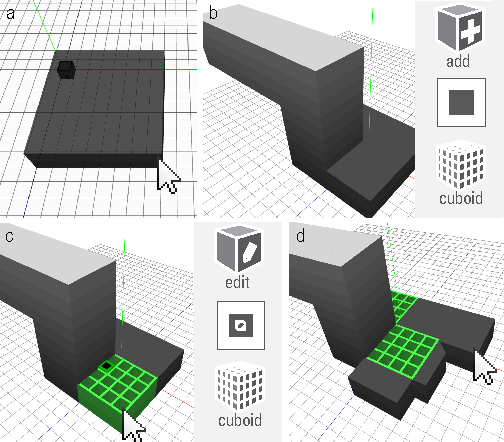
\includegraphics[width=\textwidth]{chapters/metamaterial-mechanisms-FIG/21-editor-walkthrough.pdf}
    \caption[Short figure name.]{Walkthrough of the creating door latch mechanism. The UI elements on the right show the active tools for the respective interaction steps.
    \label{fig:21-editor-walkthrough}}
\end{figure}

\subsection{Simulating deformation}

Users now verify their design directly from within the editor, as illustrated by Figure \ref{fig:22-simulation-walkthrough}. (a) They select the anchor tool and use it to place a few anchor points at the bottom, indicating that the door latch is rigidly connected to the doorframe there. (b) Now, they use the force tool to apply a force to the door handle. Users attach a force arrow to one of the handle’s cell vertices. As users are building up the force by dragging the force tool the system already responds by showing the resulting deformation of our door latch. 

\begin{figure} [h]
    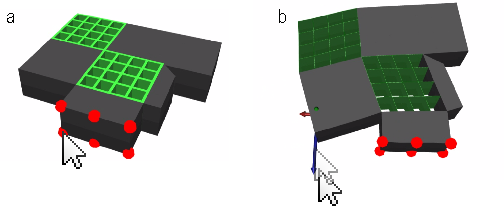
\includegraphics[width=\textwidth]{chapters/metamaterial-mechanisms-FIG/22-simulation-walkthrough.pdf}
    \caption[Short figure name.]{To simulate the deformation in real-time in the editor, (a) users set anchor points and (b) adjust forces using the force tool. 
    \label{fig:22-simulation-walkthrough}}
\end{figure}

\subsection{Multiple dimensions}
While the door latch mechanism actuates in only two dimensions, our editor also supports placing mechanisms in 3 dimensions. The latch mechanism shown in Figure \ref{fig:23-3D-object}, for example, combines a horizontal hinge array (blue) and a vertical hinge array (green) in order to create a mechanism that users operate by pressing down, sliding over, and releasing. 

Our editor color-codes mechanisms automatically according to their orientation in space. This is intended to provide users with a fast overview of the main dimensions of action in their devices and to help recognize hinge arrays from odd viewing angles. In the latch example, green denotes ``shearing on the x/z plane" and blue stands for ``shearing on the x/y plane". Analogously, red stands for ``shearing on the y/z plane".

\begin{figure} [h]
    \includegraphics[width=\textwidth]{chapters/metamaterial-mechanisms-FIG/23-3D-object.pdf}
    \caption[Short figure name.]{This latch requires the ability to shear on two planes, i.e., on the x/z plane denoted in green, and on the on x/y plane indicated in blue.
    \label{fig:23-3D-object}}
\end{figure}

Note that hinge arrays can overlap. In this case, cells at the intersection bear the combination of all holes. These cells are rendered as the additive mixture of the involved colors, such as yellow, for cells at the intersection between green and red.


\subsection{Integrating other metamaterial systems}

The shear cell is the main element that enables metamaterial mechanisms. However, to allow for the integration with metamaterials by other researchers, the editor can be extended to allow for other cell types. 

In order to allow users to explore their own cell types, we offer the advanced panel shown in Figure \ref{fig:24-advanced-cell-builder}. Users compose cells from individual edges by selecting the respective edges. The editor automatically adds all custom cells used in the current model to the cells panel for quick reuse. 

\begin{figure} [h]
    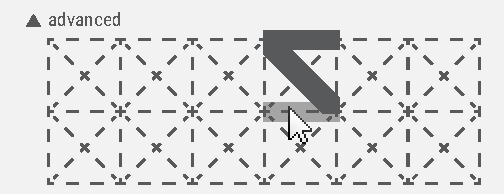
\includegraphics[width=\textwidth]{chapters/metamaterial-mechanisms-FIG/24-advanced-cell-builder.pdf}
    \caption[Short figure name.]{Users compose custom cells by adding individual edges in the ``advanced" panel.
    \label{fig:24-advanced-cell-builder}}
\end{figure}

Furthermore, users can also create and store groups of cells, for example to create auxetic materials \cite{Saxena2016}, as shown in Figure \ref{fig:25-advanced-cell-groups}. Since metamaterial mechanisms adhere to the standard structure of 3D cell grids that is common for metamaterials, they integrate with earlier research \cite{Panetta2015, Schumacher2015}.

\begin{figure} [h]
    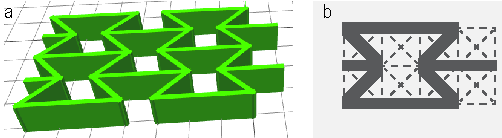
\includegraphics[width=\textwidth]{chapters/metamaterial-mechanisms-FIG/25-advanced-cell-groups.pdf}
    \caption[Short figure name.]{Users add groups of cells, here they create an auxetic material from a $4 \times 2$ group of cells.
    \label{fig:25-advanced-cell-groups}}
\end{figure}


\subsection{System Implementation}
\label{section:mechanisms-editor}

In the following, we provide details on the internal processes implemented in our metamaterial mechanisms editor.

\subsubsection{Editor (.js)}
Our 3D editor is based on WebGL and uses three.js. Internally, the editor creates a dictionary of cells that can be accessed using their position on the grid. Each cell is defined by the 8 vertices making up its bounding box by and the edges that define how the vertices are connected. Note that not all 8 vertices need to be connected by edges. 

All vertices lie on our uniform 3-dimensional grid. To generate the 3D cells' structures, i.e., to generate 3D beams from 1D edges, we apply an offset to the vertices’ positions on the GPU. Since WebGL does not offer geometry shaders, we use a vertex shader and pass the offset direction and the cell’s position with each vertex. The 8 vertices that form a beam are offset uniformly from the two edge vertices on the GPU. To pass additional information about the color and thickness of beams to the shader, we generate a texture where each pixel holds these data for one cell. The color maps directly and the thickness is encoded in the alpha component. In the shader, every vertex looks up its thickness in the texture and calculates the offsets for the new vertices that render a beam from an edge. This enables us to emulate a geometry shader in WebGL and perform all geometry processing on the GPU, which keeps the user experience of our editor smooth.

\subsubsection{Simulation (C\#)}
For simulating the deformation of the user’s cell structure, we use the finite elements solver \textit{karamba}\footnote{\url{http://www.karamba3d.com/}}, which is a plugin-for Grasshopper/Rhinoceros. We implemented a custom C\#-Grasshopper-component that receives the mesh data (vertices and edges) and the data for the simulation (anchored vertices, force and vertex where the force applies) via a web socket connection. When the simulation is complete, a second custom component receives the transformed mesh vertices and sends them back to the editor. The vertices are kept in the same order within the array as they were received from the editor. We run the simulation on a separate machine to keep the editor running smoothly. 

Maintaining the order of the vertices is important to enable geometry processing on the GPU. In the editor, we generate another texture and store the transformed vertices, where XYZ is mapped to RGB. The shader knows the vertex' undeformed position on the grid and looks up the deformed position in the texture.

Depending on the size of the object that is simulated, solving for the deformation can lead to perceivable delays. To compensate for this, our editor interpolates the deformation while the response from the simulation is pending. To do so, we pass the last force where we received the transformation from the server, and the current force that was submitted to the simulation and interpolate the vertex transformation linearly.

\subsubsection{Import \& Export}

\todo{correct}
Users can import mesh geometries directly into our editor. We voxelize the meshes using \textit{binvox}\footnote{\url{http://www.cs.princeton.edu/~min/binvox/}}  according to the cell size that the user defined.

\todo{correct}
We generate an .stl file for the user that is ready to be 3D printed. Our export is based on OpenJSCAD. In this step, we refine the cell structure from the simplified editor view to our beams with stiff members and thin living hinges. For every edge that belongs to a shear cell, we create a beam with a thick part in the middle. Edges that are part of rigid cells are generated as simple straight beams. Finally, we use OpenJSCAD's built-in render engine, which we invoke directly from our 3D editor to perform the union operations and generate the .stl file.


\subsection{Software architecture}

\todo{describe}

\begin{figure} [h] 
    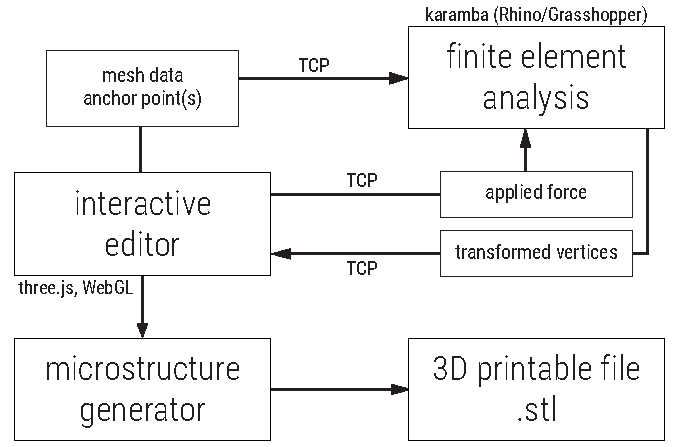
\includegraphics[width=\textwidth]{chapters/software-FIG/simple-software-architecture.pdf}
    \caption[Short figure name.]{\todo{software-architecture}
    \label{fig:simple-software-architecture}}
\end{figure}






%-----------------DIGITAL-----------------

\section{Adding digital metamaterials}
To allow expert users to create and fabricate objects from digital metamaterials, we implemented a specialized 3D voxel-style editor, which is based on the editor for metamaterial mechanisms shown in Section \ref{section:mechanisms-editor}. The main intent is to allow users to draw signal paths and verify them within the editor (Figure \ref{fig:27-editor-interface}). We support users by allowing them to enter simple logic functions, which our editor converts to cell arrangements that implement that function.

While the editor is built to help users design digital metamaterials efficiently, knowledge about signals and logic remains necessary, i.e., this editor is for expert users. 

\begin{figure} [h]
    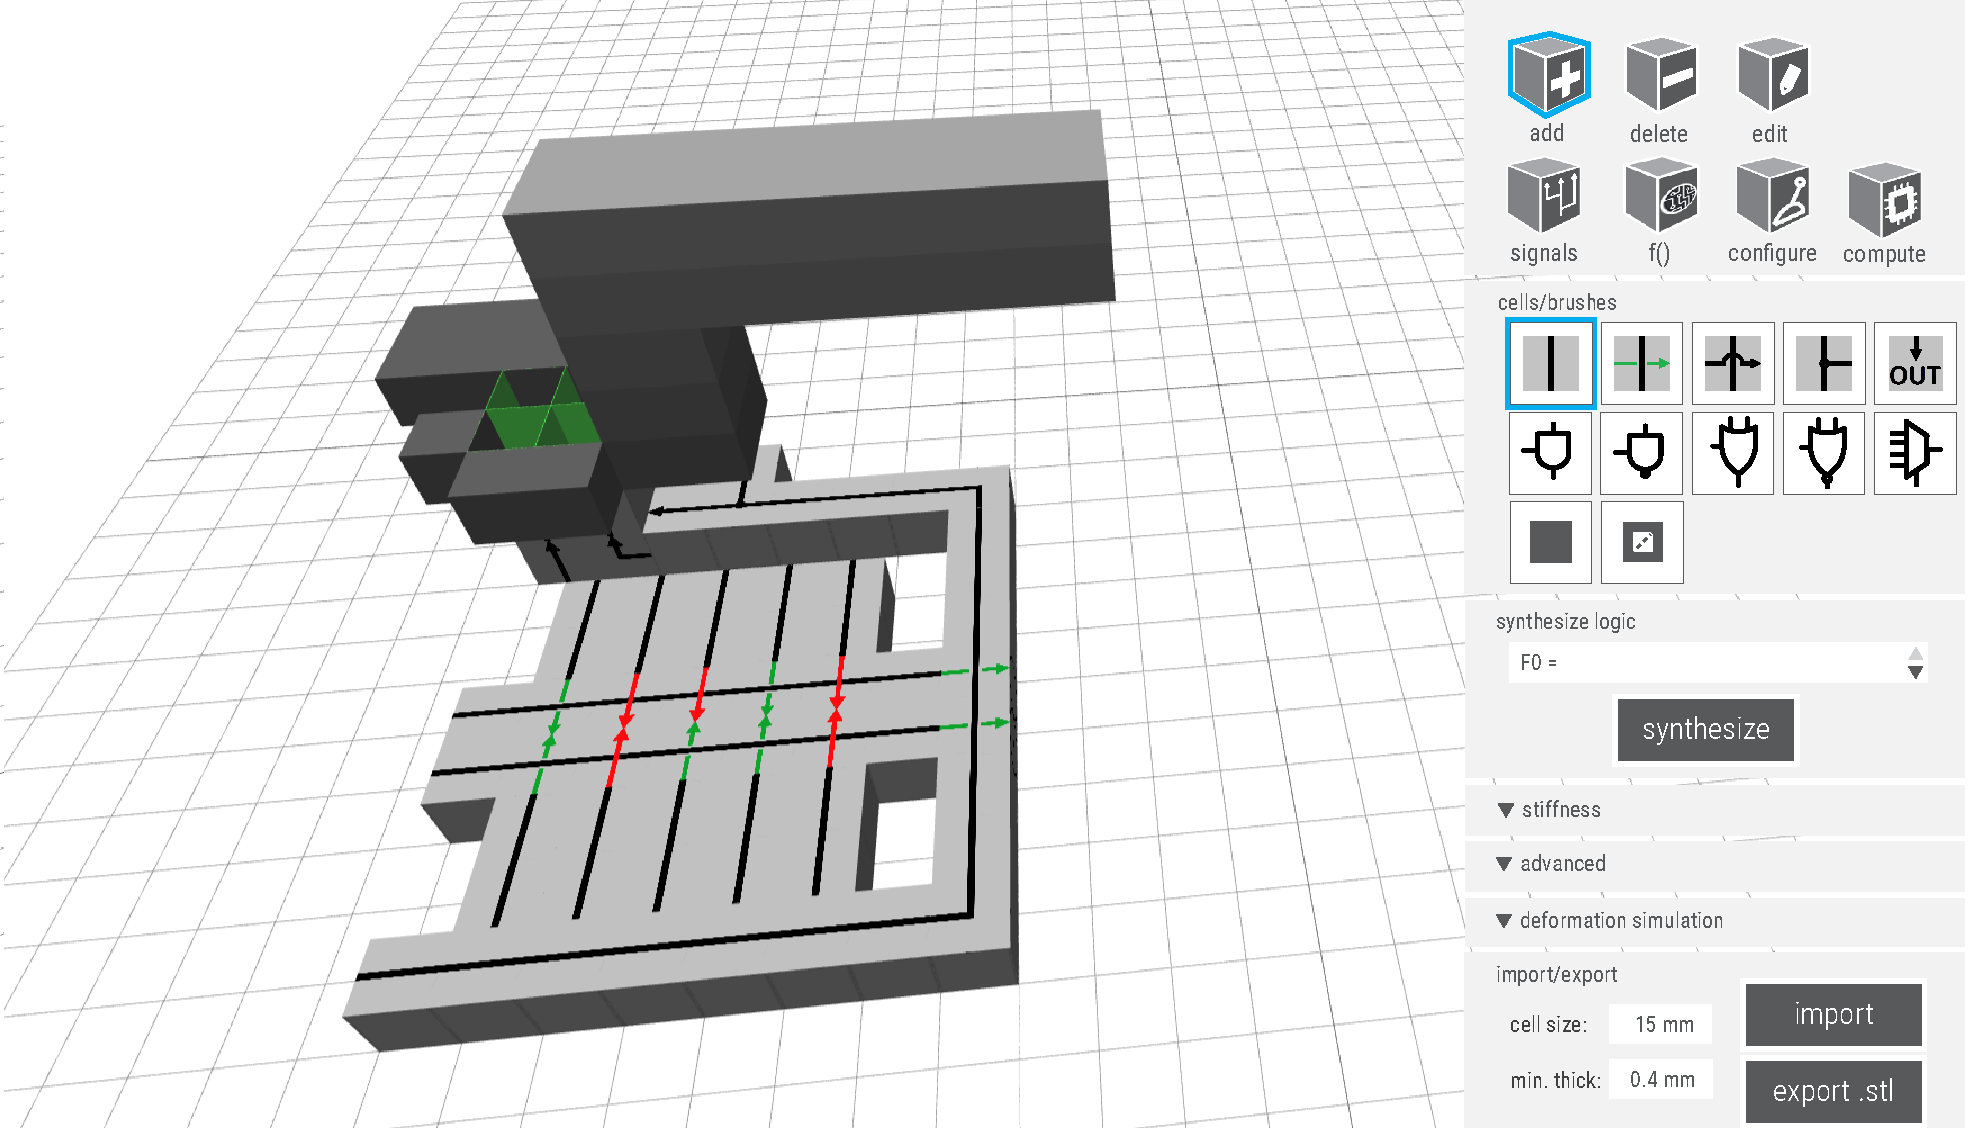
\includegraphics[width=\textwidth]{chapters/digital-metamaterials-FIG/27-editor-interface.pdf}
    \caption[Short figure name.]{Our editor helps users create digital metamaterials.
    \label{fig:27-editor-interface}}
\end{figure}

\subsection{User interaction}
Figure \ref{fig:28-editor-draw-signals} illustrates how users create the door lock example from Figure 1. (a) They first draw the signal line that evaluates the upper 5 digits by dragging over the ground plane using our ``draw signals" tool. (b) Then, using the same tool, they draw signals perpendicular to the first signal line. (c) When the two signals cross, the editor automatically draws a gate cell. (d) They do the same for the lower row of digits. (e) In this example, users manually configure the gate cells using the ``configure", i.e., they change the initial state of 5 gate cells from initially `pass' to `block' by clicking on the respective gate cell. (f) The configured gate cells implement the key code for the lock. 

Users continue by adding the evaluation line, the AND gate and the output cells, which will move the bolts. Finally, they model the analog door latch mechanism on top of the digital metamaterial. 

\begin{figure} [h]
    \includegraphics[width=\textwidth]{chapters/digital-metamaterials-FIG/28-editor-draw-signals.pdf}
    \caption[Short figure name.]{(a) Users draw the signal routing using the ``draw signals" tool. (b) Once they cross an existing signal route, (c) the editor automatically draws a gate cell. (d) After creating all cells for the digit evaluation, (e) users set the initial states of the gate cells using the ``configure" tool (f) to define the key code.
    \label{fig:28-editor-draw-signals}}
\end{figure}

Figure \ref{fig:29-editor-verify-signals} shows how users verify the signal transmission in our custom editor. They first charge the cells by selecting the ``compute" tool. The editor visualizes charged cells by turning the signal lines blue. Clicking on a cell, as shown in Figure \ref{fig:29-editor-verify-signals}a, sets a signal off. The impulse runs through the cells, being visualized in yellow at the currently active cell. After the impulse has passed a cell, the signal path is shown in black again, because the cell is back in its relaxed state (Figure \ref{fig:29-editor-verify-signals}b). To verify the whole computational assembly, users trigger the inputs first and then the evaluation signal, as they do on the 3D printed object. They subsequently watch if the signal runs all the way through to the door. If not, they see where the signal stopped and can correct the error. 

\begin{figure} [h]
    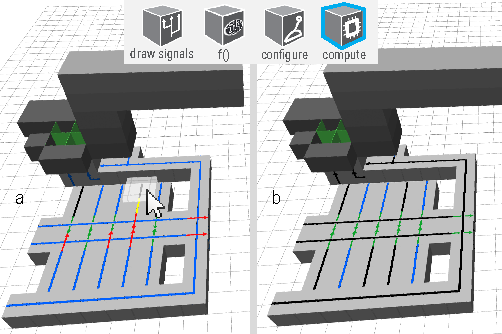
\includegraphics[width=\textwidth]{chapters/digital-metamaterials-FIG/29-editor-verify-signals.pdf}
    \caption[Short figure name.]{Users can verify their logic and signal routing. They first charge all springs, then (a) they click the inputs to trigger the signal there, and lastly (b) they trigger the evaluation line and find that the signal passes all the way through to the latch.
    \label{fig:29-editor-verify-signals}}
\end{figure}

To help users create logic functions efficiently, e.g., by avoiding the need for manual configuration of cells, we allow users to input logic functions. Figure \ref{fig:30-editor-synthesize-cells} shows an example, where users enter the function `A \& {\textasciitilde}B \& C \& D \& {\textasciitilde}E' and click ‘synthesize’. Then, they indicate where the synthesized cell arrangement shall be positioned by simply clicking on the grid. Our editor automatically synthesizes the cells that implement the entered logic functions. 

\begin{figure} [h]
    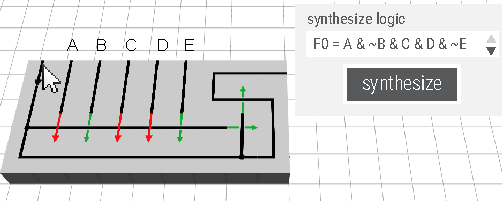
\includegraphics[width=\textwidth]{chapters/digital-metamaterials-FIG/30-editor-synthesize-cells.pdf}
    \caption[Short figure name.]{Users enter the function `A \& {\textasciitilde}B \& C \& D \& {\textasciitilde}E', and indicates the location by clicking on the grid. Our editor responds by automatically inserting the corresponding cells.
    \label{fig:30-editor-synthesize-cells}}
\end{figure}


\subsection{Implementation}
We build on the metamaterial mechanisms voxel-style editor and extend it to allow users to draw signal routes and to input logic functions. Our extension of the editor is based on a node.js javascript framework, using the three.js graphics framework and WebGL for rendering the basic geometries.

Rendering of 3D-printable .stl files was done in modular hierarchical OpenSCAD script files. The editor simply exports the cell geometries as OpenSCAD script commands to render a cell with the specific parameters.

\subsubsection{Drawing signal paths}
%\paragraph{Drawing signal paths} 
Drawing signal paths is realized through a freeform line tool that places appropriately connected cells following the cursor. We use a pathfinding library for 3D\footnote{\url{https://github.com/schteppe/PathFinding3D.js}} that provides the A\* pathfinding algorithm to simplify connecting cells via a signal line by finding the shortest available path while crossing existing signals where necessary.


\subsection{Synthesizing cell arrangements from boolean expressions}
%\paragraph{To synthesize cell arrangements}
To generate cell arrangements of minimal size that implement a user-defined logic function, we use a version of the Espresso heuristic logic minimizer\footnote{\url{https://embedded.eecs.berkeley.edu/pubs/downloads/espresso/index.htm}}. 

The logic minimizer parses the user text input, minimizes the described input function and returns it in its disjunctive normal form. This minimized DNF is parsed a second time by our editor to identify its terms and literals, which are used to create a very compact cell arrangement that forms a disjunction of minterm conjunctions. A minterm is a minimal conjunction of the input literals that returns true. This means that an array of signals representing the disjunctions of the function is run in parallel. All input variables of the function intersect and potentially block these lines, forming conjunctions along each of the parallel lines. The combined arrangement implements the function as a whole. To choose the most succinct cell representation of the function, we also minimize the negated input function and negate its result again directly on the cell level. The cell arrangement variant that requires the least cells to implement the input function is constructed and placed in the editor at the last user-selected cell location.

The logic minimizer runs in a separate python virtual environment using the PyEDA\footnote{\url{http://pyeda.readthedocs.io/en/latest/index.html }} library for electronic design automation. This python server is queried via HTTP requests to a REST architecture and replies with minimized functions to logic functions encoded in the request-URL.

%\subsection{Simulating signal flow}











%-----------------TEXTURES-----------------


\section{Editing Textures to Provide Output}

Figure \ref{fig:16-editor-ui} shows the interactive editor we built to assist designers in creating textures based on metamaterials. Here, we see a user creating a block that when pushed displays a zigzag texture on the top. 

\begin{figure} [h]  
    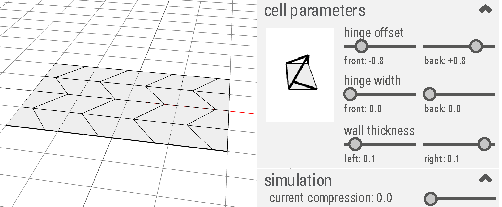
\includegraphics[width=\textwidth]{chapters/metamaterial-textures-FIG/16-editor-ui.pdf}
    \caption[Short figure name.]{Our editor assists users in creating metamaterial textures. Users adjust the cell geometry using sliders and lay the cells out on the grid.
    \label{fig:16-editor-ui}}
\end{figure}


\subsection{User interaction}

In the interactive editor, we exploit the fact that the fold cell is fully parameterized. Users can set all parameters (Figure \ref{fig:16-editor-ui}, \textit{right}), for example hinge offset, width and wall thickness, simply by dragging the individual sliders. An interactive preview of a cell in its actuated state (Figure \ref{fig:16-editor-ui}, \textit{left from the parameters}) allows users to see how the cell will look like once placed and actuated. After setting all parameters, users can arrange the cells on a regular grid to create textures from metamaterials. 

Our editor runs in a browser. It is based on the editor for metamaterial mechanisms, which is built using node.js (a Javascript runtime framework) and utilizes the three.js library for rendering. 

\subsection{Previewing textures by means of simulation}

The editor offers a preview of the resulting texture based on the user's current metamaterial design. They can interactively preview the different textures, which result from different compression rates by simply dragging the slider (Figure \ref{fig:17-editor-simulation}) that specifies the current compression. The deformation of the textures is rendered in real-time.

\begin{figure} [h]  
    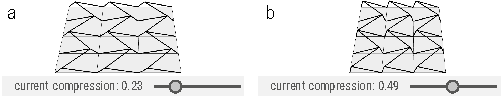
\includegraphics[width=\textwidth]{chapters/metamaterial-textures-FIG/17-editor-simulation.pdf}
    \caption[Short figure name.]{Users interactively preview their textures by dragging the slider that sets the simulated compression. 
    \label{fig:17-editor-simulation}}
\end{figure}

The simple kinematic simulation that we implemented in our editor allows for previewing, in real-time, how the designed textures fold up when the material is compressed via a GUI slider. Our simulation calculates only geometric transformations by simple propagation, i.e., as a cell compresses, its members move, in turn, these members move the neighboring cell's members, and so forth. 

Note that at this stage our simulation does not take material properties into account. We opted for this approach as it allows for an interactive simulation (at 30 fps) compared to, e.g., finite element analysis, which is computationally more expensive and therefore slower, but more accurate. 


\subsection{Generating a printable file}

To simplify the process of creating a texture based on metamaterials, our editor only requires users to choose how the surface of the cell should fold to form their texture. In fact, the remainder of the 3D object, e.g., its internal structure beyond the top layer, is generated by our editor when users export the final texture. 

We derive the parameters for the remainder cell geometry from the user defined hinge positions. The wall thickness is derived from the hinge offsets. For a diagonal hinge, we gradually decrease the thickness of the middle connector towards the top so that it connects only to the center of the texture geometry with minimum widths of $0.3\, \mathrm{mm}$. After having created the cell body for the fold cell, we repeat this structure until the user-defined volume is filled. Finally, this geometry is exported into a 3D printable .stl file.


\subsection{Limitations of the interactive editor}

Our editor only allows creating objects with simple geometries, i.e., planar, curved, and cylindrical. Our current kinematic simulation enables real-time interaction at the expense of offering more simplistic results. These, however, preview all the textures we demonstrated correctly. 


% \section{Software architecture}

% \todo{if time: make new, full diagramm of how the completely integrated editor would look like}

% \begin{figure} [h] 
%     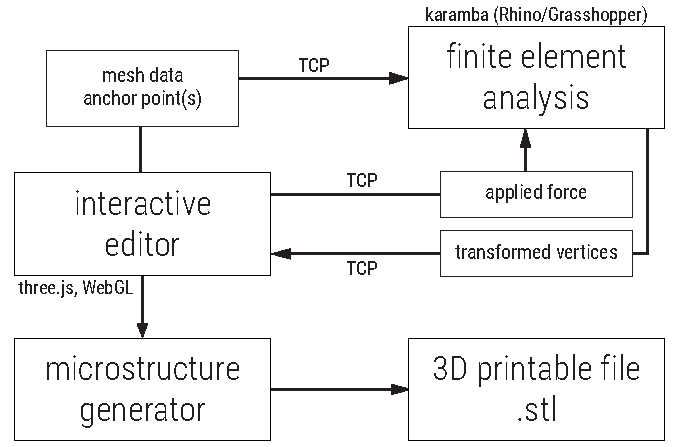
\includegraphics[width=\textwidth]{chapters/software-FIG/simple-software-architecture.pdf}
%     \caption[Short figure name.]{\todo{simple-software-architecture}
%     \label{fig:simple-software-architecture}}
% \end{figure}


% \section{Discussion}
% \todo{while it is not all tied in together, here is how it should look like}





